\documentclass[11pt,oneside]{amsart}
\usepackage{geometry}
\geometry{letterpaper}
\usepackage{graphicx}
\usepackage{caption}
\usepackage[singlelinecheck=off,justification=raggedright]{subcaption}
% Change subfigure letters to uppercase
\renewcommand{\thesubfigure}{\Alph{subfigure}}

\usepackage{amssymb}
\usepackage{epstopdf}
\usepackage{natbib}
\usepackage{color}
\usepackage{multirow}
\usepackage{setspace}
\usepackage{xcolor}
\usepackage{tikz}
\usepackage{mathtools}
\usepackage{bbm}
\usepackage{rotating, graphicx}



\setlength{\topmargin}{0in}
\setlength{\oddsidemargin}{0in}
\setlength{\textwidth}{6.5in}
\setlength{\textheight}{8.85in}

\RequirePackage{lineno}
\onehalfspacing
\DeclareGraphicsRule{.tif}{png}{.png}{`convert #1 `dirname #1`/`basename #1 .tif`.png}

\bibpunct{(}{)}{,}{a}{}{;}

\newcommand{\E}{\mathbb E}
\newcommand{\Prob}{\mathbb P}
\newcommand{\var}{\text{Var}}
\newcommand{\cov}{\text{Cov}}
\newcommand{\corr}{\text{Corr}}
\newcommand{\nm}{\tilde n_t}
\newcommand{\ns}{\hat n_t}
\newcommand{\nr}{p_t}
\newcommand{\nmtau}{\tilde n_\tau}
\newcommand{\nstau}{\hat n_\tau}
\newcommand{\nrtau}{p_{\tau}}
\newcommand{\Stree}{\mathcal H}
\newcommand{\Gtree}{\mathcal G}
\newcommand{\Top}{\mathcal T}
\newcommand{\Data}{X}
\newcommand{\D}{\mathcal D}
\newcommand{\N}{\mathcal N}
\newcommand{\tcb}{\textcolor{blue}}
\newcommand{\defeq}{\vcentcolon=}

\begin{document}

\linenumbers

\theoremstyle{plain}
\newtheorem{theorem}{Theorem}[section]
\newtheorem{lemma}[theorem]{Lemma}
\newtheorem{corollary}[theorem]{Corollary}
\newtheorem{proposition}[theorem]{Proposition}
\newtheorem{definition}[theorem]{Definition}

\title{A Markov Model of the Coalescent with Recombination and Population Substructure}

\maketitle

\section{Abstract}
\label{Section: Abstract}

Different biological phenomena can leave similar signatures in the genomic data. This project explores how recombination and population substructure can lead to patterns of ancestry across different places in the genome that could appear similar to the signatures of other biological phenomena, such as horizontal gene transfer. In this project, we develop a framework for simulating genomic data under a neutral model with population substructure and recombination. We extend the model of \cite{SimonsenChurchill1997}, a Markov model of the coalescent with recombination between a discrete number of loci, to also include two subpopulations with a symmetric migration rate between them. We describe the state space and transition matrix of this model. Using the transition matrix, we find that the probability of equal time to the most recent common ancestor at each loci decreases with decreasing migration rate and increasing recombination rate. The model described in this paper is a first step towards developing a statistic to discriminate between the genomic signature of horizontal gene transfer and the possible genomic signature of recombination and population substructure.

\section{Introduction}
\label{Section: Introduction}

Incomplete lineage sorting refers to the neutral process by which ancestral lineages from a population fail to coalesce more recently in time than the ancestral population split with one or more other populations \citep{DegnanRosenberg2009}. Incomplete lineage sorting creates the possibility that a lineage, $a1$, from population $A$, shares a common ancestor with another lineage, $b1$ from population $B$, more recently than $a1$ shares an ancestor with other lineages from population $A$. Due to incomplete lineage sorting, when species are closely related, the topology of the sample genealogy (the gene tree), can differ from the topology of the species phylogeny (the species tree) \citep{Hudson1983, Tajima1983}.

Recombination can lead to variation in the genealogy of a sample across loci. Because gene trees can differ from species trees and gene trees can vary across different loci, some loci in the genome may have genealogies which accord with the overall species tree, while neighboring loci do not. 

We will refer to the phenomena in which the local gene tree does not accord with the topology of the overall species tree as \textit{gene-species tree discordance}. With recombination and incomplete lineage sorting, gene-species tree discordance can vary across the genome. For example, the relationship between humans, chimps, and gorillas varies across the genome \citep{Dutheiletal2009}. The species tree for humans, chimps, and gorillas is considered to be \mbox{\{\{human, chimp\}, gorilla\}}. While \mbox{\{\{human, chimp\}, gorilla\}} is the topology over most of the genome, at some loci, the topology relating the samples is \mbox{\{\{human, gorilla\}, chimp\}} or \mbox{\{\{chimp, gorilla\}, human\}}.

Beyond incomplete lineage sorting during descent from a shared ancestral population, gene-species tree discordance can also be evidence for other biological phenomena. Some methods for identifying horizontal gene transfer rely on identifying tracts of the genome in which gene-species discordance is adjacent to other regions of concordance between the gene tree and species tree \citep{Ochman2001}. Modeling different processes which lead to gene-species tree discordance can be utilized to improve inference methods for differentiating between them \citep{RuthsNakleh2005}. In this project we are interested in modeling how variation in gene-species tree discordance across different loci can arise in a neutral model.

\subsection{A coalescent model}
\label{subsection: a coalescent model}

\cite{SlatkinPollack2006} introduced a framework for analyzing the probability of gene-species tree discordance in a simple three-species coalescent model with recombination. \cite{SlatkinPollack2006} considered the case of two loci and a sample of one individual per species. Their model utilized a spatially discrete model of the coalescent with recombination introduced by \cite{SimonsenChurchill1997}. The probability of gene-species tree discordance at each of the loci depends on the number of lineages present in the ancestral population.% The number of loci present in the ancestral population and the relationship between the two loci is determined by both the length of the internal branch ($T = t_2 - t_3$) as well as the recombination rate ($\rho$) between the two loci.

\cite{SlatkinPollack2008} described a second model in which ancestral population substructure increases the probability of gene-species tree discordance. They showed how even in a simple model, extreme substructure within the ancestral population can lead to a discordant gene tree topology that is more likely than the concordant topology. \cite{DeGiorgioRosenberg2016} demonstrated that this discordance due to a structured ancestral population can introduce challenges for several different phylogenetic inference algorithms.

A simple demographic history which could lead to the scenario of increased gene-species tree discordance consists of three modern day populations $A$, $B$, and $C$ with the topology $((A, B)C)$. In the shared ancestral population between $A$ and $B$, which is not ancestral to $C$, structure persists between $A$ and $B$. Further back in time, in the ancestral population which includes $A$, $B$, and $C$, population structure continues to persist between $A$ and $B$, but the ancestors of  $B$ and $C$ mix and have no population structure. In this context, \cite{SlatkinPollack2008} demonstrated that the discordant gene tree topology $(A(BC))$ can increase in probability above the probability of the concordant topology $((AB)C)$. Figure \ref{Figure: Slatkin and Pollack 2008} illustrates this scenario.

%% FIgure 1
%% \label{Figure: Slatkin and Pollack 2008}

In the model of \cite{SlatkinPollack2008}, the number of lineages in a population at a given time point is represented as a continuous Markov process.

\section{Extending the model}
\label{Section: Extending the model}

In the current project, we are interested in incorporating recombination into the model suggested by \cite{SlatkinPollack2008}, in which population substructure can increase the probability of gene-species tree discordance. We use a Markov model of the coalescent that explicitly incoporates both recombination with discrete loci and population substructure, to model a neutral process in which the probability of gene-species tree discordance can vary at different loci.

As \cite{SlatkinPollack2006} demonstrated, Markov models of genealogies at discrete loci are useful for modeling ancestry in the context of changing demographic history. To explicitly model recombination and migration in our model, we build upon the model described by \cite{SimonsenChurchill1997}. 

In the first part of this project, we delineate the state space and transition probabilities of a coalescent model with recombination and population substructure for two loci with both two and three individuals. We have created a program in \texttt{python} to generate these state spaces and the associated diagrams that describe them for general sample size, $n$. We also introduce an analytical formula for the size of the state space for two loci, two subpopulations, and general $n$ samples.

Following the analysis of \cite{SimonsenChurchill1997}, we find the probability of different tree heights between the two loci when there are two lineages present at each locus in the model. With two individuals and two loci, \cite{SimonsenChurchill1997} demonstrate how a model of recombination between two loci can lead to different coalescence times in the genealogies at each locus. When the demographic features of the population change over time, such as in a three-species model, different timing of coalescent events between lineages associated with each locus could lead to scenarios in which the coalescence events for different loci occur in different regimes of the demographic model, e.g. before or after a population splits into two. This scenario leads to the possibility that the joint probability that two loci have the same topology depends on the recombination level and the ancestral population substructure.

This project is the first step toward the goal of modeling the effect of population substructure on gene-species concordance across loci. The transition matrix and state space described in this project could be used in future projects to expand the Markov model of \cite{SlatkinPollack2008} to explicitly incorporate recombination and analyze the probability of different loci falling into different topology classes due to incomplete linkage, such that their coalescent times are not entirely correlated.

%\clearpage

\section{Markov Model of Coalescent with Recombination and Population Substructure}
\label{Section: recombination and migration}

\subsection{State space and transition matrix for model with recombination but no population substructure}
\label{Subsection: recomb}

To delineate the state space and transition matrix of a Markov model of the coalescent with recombination, we build from the model of \cite{SimonsenChurchill1997}. The state space of the process described by \cite{SimonsenChurchill1997} characterizes the numbers of lineages present at each locus. Similar to the standard coalescent model, the process begins in the present and progresses backwards in time.

Similarly to the standard coalescent model, in the \cite{SimonsenChurchill1997} model, a coalescence corresponds to an individual producing two offspring forward in time. However, because the model incorporates recombination, it is possible that an individual produces two offspring, but that one or both offspring only inherit one of the two loci from the individual of interest due to recombination. Introducing recombination into the model also introduces the possibilty that the two loci which are ancestral to the present-day individual recombined onto the same haplotype from two different individuals. Figure \ref{Figure: coalescence and recombination}(A) illustrates how, thinking forward in time, individuals can produce offspring that only inherit one of the two loci or that inherit both; these events can be considered coalescences between haplotypes that are ancestral at one or both loci. Figure \ref{Figure: coalescence and recombination}(B) illustrates how, thinking forward in time, loci ancestral to the present day sample can recombine onto the same haplotype from two individuals who only have one locus ancestral to the present-day sample. Coalescence and recombination define the transitions between states in the Markov process.

%% Figure 2
%% \label{Figure: coalescence and recombination}

Using the terminology from \cite{SimonsenChurchill1997}, the states of the Markov process represent the number of lineages present for each locus by a unique tuple $(i, j, k)$. We define $i$ as the number of ``left type" lineages, those that are ancestral to the present day sample at the left hand locus but not the right (represented as a circle in Figure \ref{Figure: terminology}(A)). Similarly $j$ represents the number of ``right type" lineages, those that are ancestral to the present day sample at the right locus, but not the left (represented as a square in Figure \ref{Figure: terminology}(B)). Lastly, $k$ represents the number of ``double type" lineages, those that are ancestral to the present day sample at both loci (represented as a circle in Figure \ref{Figure: terminology}(C)). Note that a haplotype which is ancestral to only one locus has some other allele at the other locus, but we are only interested in tracking the genealogy at loci which are ancestral to the present day sample.

%% Figure 3
%% \label{Figure: terminology}

The transitions between the states in the \cite{SimonsenChurchill1997} model are either coalescence or recombination events. In a recombination event, one double becomes a right type and left type (see Figure \ref{Figure: coalescence and recombination}(B)). The population recombination rate, $R = Nr$, represents the rate at which two lineages which are each ancestral at opposite loci recombine onto the same haplotype, $r$, scaled by the number of haplotypes in the population, $N$. In a recombination event, $k$ decreases and both $i$ and $j$ increase. In a coalescent event, a double type can coalesce with a double ($k$ decreases), a left type ($i$ decreases), or right type ($j$ decreases) or a right and left type can also coalesce into a double ($i$ and $j$ decrease, $k$ increases) (see Figure \ref{Figure: coalescence and recombination}(A)). Another type of coalescent event can occur in which two haplotypes which are ancestral to the sample only at one locus coalesce. \cite{SimonsenChurchill1997} model this possibility as two right types coalescing to one right type ($i$ decreases) or two left types coalescing to one left type ($j$ decreases). The coalescence rates are determined by the number of lineages present of each type. As in the standard coalescent model, \cite{SimonsenChurchill1997} assumes that the probability of simultaneous events is small enough to ignore. Figure \ref{Figure: recombination diagram} illustrates how the Markov chain describes the genealogy of the process.

% Figure 4
% \label{Figure: recombination diagram}

Similar to the standard coalesccent model, \cite{SimonsenChurchill1997} define a starting state with $n$ lineages. In the starting state, for each individual both loci are part of the genealogy so all $n$ lineages are in double types. As lineages coalesce, the total number of lineages decreases at each locus. Recombination does not change the total number of lineages, only changing whether or not both loci are on the same haplotype (in a double type) or on two different haplotypes (a right type and left type). At any given time, the number of lineages, $\nu_{r}$, which are ancestral to the present day sample at the right locus must be contained in a right type or a double type. Similarly the number of lineages, $\nu_{\ell}$, ancestral to the present-day sample at the left locus must be in a left type or a double type. As in the standard coalescent model, the number of lineages decreases from $n$ to $1$, so $1 \leq \nu_r \leq n$ and $1 \leq \nu_{\ell} \leq n$. Therefore the following equations define the state space,
\begin{align}
1 &\leq i+k \leq n \label{Eqn: i + k leq n} \\
1 &\leq j+k \leq n \label{Eqn: j + k leq n}  \\
0 &\leq i,j,k \leq n \label{Eqn: all geq 0}
\end{align}

\cite{SimonsenChurchill1997} consider the state space for $n = 2$ fom eqs.~(\ref{Eqn: i + k leq n})--(\ref{Eqn: all geq 0}). This computation yields 9 total states. We illustrate the state space diagram with transitions in Figure \ref{Figure: n = 2 recomb}.

% Figure 5
% \label{Figure: n = 2 recomb}

 \cite{SimonsenChurchill1997} also describe how to extend their model to other numbers of loci and samples but only illustrate the state space and transition matrix explicitly for $n = 2$. For two loci and general $n$, they show that the number of states is $n(2n^2+9n+1)/6$. 

For $n = 3$ the number of states is 23. Using, \texttt{python}, we delineate the case of $n =3$ case explicitly. We generated the states based on the allowable tuples given in inequalities (\ref{Eqn: i + k leq n})--(\ref{Eqn: all geq 0}). We generated the transition matrix by considering the transitions- recombination or coalescence- which lead to valid states. We generated a diagram using the software \texttt{graphviz}. For $n=3$, we illustrate the state space diagram with transitions in Figure \ref{Figure: n = 3 recomb}. 

% Figure 6
% \label{Figure: n = 3 recomb}
	
\subsection{Extending the model to include population substructure.}
\label{Subsection: recomb and mig}

To extend this model to include population substructure, we consider a model with two populations with a migration rate, $M = Nm$, where $N$ is the number of haplotypes in each subpopulation and $m$ is the rate of migration for an individual haplotype to migrate to the other subpopulation. 

Recombination and coalescent events change the number of lineages of each type present in one population only. Two lineages can only coalesce at a given time if they are currently in the same population. A double type can recombine into a right type and left type, both of which remain in the same population. Any type of lineages (right type, left type, or double type) can migrate. As in the model with only recombination, we assume that the resulting lineages remain in the same population given that coalescence, recombination, and migration are so rare that we can ignore the possibility of two events occuring simultaneously.

From the nine states in the \cite{SimonsenChurchill1997} model with two samples and two loci, the extended population substructure and recombination Markov chain includes 46 states, as shown in Figure \ref{Figure: n = 2 recomb mig}. We label the states using the following terminology: \mbox{\{$iA$, $jA$, $kA$\}\{$iB$, $jB$, $kB$\}} where \mbox{\{$iA$, $jA$, $kA$\}} represents the number of lineages of right types, left types, and double types in population $A$ and \mbox{\{$iB$, $jB$, $kB$\}} represents the number of lineages of different types in population $B$.

The number of lineages in the model with recombination and no population substructure are constrained by eqs.~(\ref{Eqn: i + k leq n})--(\ref{Eqn: all geq 0}). In the model with both recombination and population substructure, we can generate all of the states by accounting for all possible population labels on the lineages in each state from the original model with recombination but no population substructure, i.e. the states are constrained by eqs.~(\ref{Eqn: i + k leq n})--(\ref{Eqn: all geq 0}) for $i = iA + iB$, $j = jA + jB$, and $k = kA + kB$.

Figure \ref{Figure: migration diagram} illustrates how the Markov chain corresponds to the coalescent process with recombination and migration.

% Figure 7
% \label{Figure: migration diagram}

% Figure 8
% \label{Figure: n = 2 recomb mig}

Ignoring topology, extending the Simonsen and Churchill model to include $n$ samples and 2 loci,  we used a combinatorial argument to find the number of states in the model given a value of $n$. 

Starting from the number of possible states from $n$ lineages in the model without substructure, we find the number of lattice point solutions to inequalities (\ref{Eqn: i + k leq n})--(\ref{Eqn: all geq 0}):
\begin{align}
& \sum^{n}_{k = 0} \sum^{n-k}_{j = 0} \sum^{n-k}_{i = 0}  \mathbbm{1}\{0 < i + k\}\mathbbm{1}\{0 < j + k\} \\
& \sum^{n}_{k = 1} \sum^{n-k}_{j = 0} \sum^{n-k}_{i = 0}  \mathbbm{1}\{0 < i + k\}\mathbbm{1}\{0 < j + k\} + \sum^{n}_{j = 1} \sum^{n}_{i = 1}  \mathbbm{1}\{0 < i\}\mathbbm{1}\{0 < j\} \\
& \sum^{n}_{k = 1} \sum^{n-k}_{j = 0} \sum^{n-k}_{i = 0}  \mathbbm{1}\{0 < i + k\}\mathbbm{1}\{0 < j + k\} + n^2
\end{align}

\noindent which simplifies to $n(2n^2+9n+1)/6$ from \cite{SimonsenChurchill1997}.

For any given tuple $(i, j, k)$ in the model with only recombination and no population substructure, we can partition the lineages into two subpopulations. Each of the $i$ left-type lineages can be in population A or population B. Because the lineages are exchangeable, placing the $i$ lineages into two non-exchangeable populations give $i+1$ total states: either 0, 1, 2, \ldots , or $i$ left-type lineages are placed in population A. Similarly, the $j$ right-type lineages generate $j+1$ states, and the $k$ double-type lineages generate $k+1$ states. The number of ways to create this partition is equivalent to counting the ways to split into two groups three series of $i$, $j$, and $k$ identical objects, because all lineages of a given type are exchangeable with the other lineages of that type and the placement of any lineage in a population is independent on the placement of other lineages. 

We have
\begin{align}
S(n) &= \sum^{n}_{k = 0} \sum^{n-k}_{j = 0} \sum^{n-k}_{i = 0}  \mathbbm{1}\{0 < i + k\}\mathbbm{1}\{0 < j + k\}(i+1)(j+1)(k+1) \\
&= \Big( \sum^{n}_{k = 1} \sum^{n-k}_{j = 0} \sum^{n-k}_{i = 0} (i+1)(j+1)(k+1) \Big) + \sum^{n}_{j = 1} \sum^{n}_{j = 1}(i+1)(j+1)\\
&= \sum^{n}_{z = 0} \Bigg( (n-z+1)\bigg[\Big(\sum^{z}_{y = 1} (y+1)\Big)^2 + \mathbbm{1}\{n-z > 0\}(1+2\bigg(\sum^z_{y = 1}(y+1)\Big) \bigg] \Bigg).
\label{Eqn: combinatorial count}
\end{align}

We used Faulhaber's formulas to simplify the expression to find the closed form expression is below.
\begin{equation}
S(n) = \frac{n^6}{120}+\frac{n^5}{8}+\frac{3n^4}{4}+\frac{55n^3}{24}+\frac{329n^2}{120}+\frac{n}{12}.
\label{Eqn: combinatorial count Fauhaber formula}
\end{equation}

For $n = 2$, we have $S(n) = 46$ and for $n=3$ we have $S(n) = 184$. The program we created in \texttt{python} generate these states and transition matrix, given the allowable states, and the allowable transitions between states- coalescence, recombination, and migration. Figure \ref{Figure: n = 3 recomb mig} shows the state space and transitions for the case of $n = 3$ model with recombination and migration.

% Figure 9
% \label{Figure: n = 3 recomb mig}

\subsection{Probability of equal tree height.}
\label{subsection: pequal tree height}

Using the transition matrix of the Markov process defined in Sections \ref{Subsection: recomb} and \ref{Subsection: recomb and mig}, we can observe the properties of the genealogical process with recombination between 2 loci in the case of $n = 2$ and $n = 3$ samples per population, with recombination between the two loci in a model with or without population structure.

In the model with no population substructure and two loci, \cite{Griffiths1981} determined an analytical formula for the probability that the two trees have equal height, i.e. that the time to the most recent common ancestor between the right and left locus are the same. This probability is recapitulated in \cite{SimonsenChurchill1997} who explored the probability of equal tree height analytically by analyzing long-term behavior of the transition matrix. This analysis enabled them to find the probability that the process never enters the states of the process in which $i + k = 1$ but $j + k > 1$ or, similarly, in which $j + k = 1$ but $i + k > 1$ . They found the probability of equal tree height to be 
\begin{equation}
\frac{9+R}{9+13R + 2R^2},
\label{Eqn: equal tree height}
\end{equation}

which decreases as $R$ increases.

% uneqht_nomig_states = ['101', '011', '210', '120', '110']
In the model with only recombination and no population substructure, if the process enters states $\{101\}$, $\{011\}$, $\{210\}$, $\{120\}$, or $\{110\}$ the tree heights will be unequal. The probability of equal tree height can be determined by finding the probability that the process never enters one of these states. %Although the relevant states for the $n = 2$ and $n = 3$ case are the same, the overall probability of tree height for these cases may differ because the rest of the state space and transitions differ.

For the model with recombination and population substructure, each state corresponds to a state from the model with recombination and no population labels. To find the probability of equal tree height for a given recombination rate, $R$, and migration rate, $M$, we can consider whether the process ever enters states $\{iA, jA, kA\}\{iB, jB, kB \}$ such that $\{iA + iB, jA, + jB, kA + kB \}$ equals one of $\{101\}, \{011\}, \{210\}, \{120\}$, or $\{110\}$. 

In the $n = 2$ case, this results in 24 states in the model with recombination and population substructure which lead to unequal tree heights between the two loci. We estimated the probability of equal tree height by running $10^4$ simulations of the Markov process for the model with recombination and population substructure with different recombination rates, $R$, and migration rates, $M$. We found that for increasing recombination rate, $R$, and decreasing migration rate, $M$, the probability of equal tree heights decreases.

At the start of the process, the two lineages begin in different subpopulations. A small migration rate increases the time in which recombination can break up the two loci onto different haplotypes because coalescences cannot occur unless there are two lineages associated with the same locus in the same population. Once the two loci are broken up, the probability of equal tree height is decreased because the two lineages will behave independently and each must migrate separately to the other population in order for a coalescence to occur. Thus, the probability of unequal tree height increases as the migration rate, $M$, decreases for a given recombination rate, $R$.

% Figure 10
% \label{Figure: pequal height}

\section{Conclusion}
\label{Section: conclusion}

In this project, we have delineated the state space and transition matrix for a two-locus coalescent model with recombination and migration for $n = 2$ and $n = 3$ lineages per population in a two-population model by extending the model of \cite{SimonsenChurchill1997}. For the $n = 2$ case, by simulating the Markov process from its transition matrix we estimated the probability of unequal tree height between the two loci.

We found that the size of the state space increases polynomially with $n$, in particular following $n^6$. The probability of equal tree height decreases with decreasing $M$ and increasing $R$. The Markov framework described in this chapter could be used to extend the model described in \cite{SlatkinPollack2008} to better understanding how neutral processes could cause the probabilities of different topologies at incompletely linked loci to differ. As described in Section \ref{subsection: pequal tree height}, population substructure increases the tree height and increases the probability that the tree heights between loci will differ compared to a model with no population substructure. 

For a demographic scenario with population substructure which changes over time, such as in the \cite{SlatkinPollack2008} model, the probabilities determining migration-- and as a consequence, coalescence-- may vary between two loci if the process at one locus is complete (i.e. one ancestor) while the other is still ongoing. In the context of the demographic schema described by \cite{SlatkinPollack2008}, population substructure also increases the probability of gene-species tree discordance. One use of our model would be to explore how an increased probability of unequal tree heights, due to the presence of population substructure, and an increased probability of gene-species tree discordance, due to the presence of population substructure, could increase the probability of gene-species tree discordance at one locus and gene-species tree concordance at the other locus. 

Modeling gene-species tree discordance in this way lays the groundwork for developing a 3-point statistic to estimate the parameters necessary to produce gene-species tree discordance in short tracts in the genome flanked by gene-species tree concordance on either side. Here, we only explore the 2 loci model with migration, but an extension to include 3 loci, could model the probability that across three loci in the genome one left most loci has a concordant topology, the middle loci has a discordant topology, and the right most loci has a concordant topology-- a genomic signature similar to that of horizontal gene transfer.


%We compared the probability of equal tree height as it changes with recombination rate for the Simonsen and Churchill model and the extended model with population structure. Simonsen and Churchill also show a scatter plot of simulated left and right tree heights given a population recombination rate, R = 2N*r = 0.723, the value for which the probabilities of equal and unequal tree heights are approximately equal to the probabilty of unequal tree heights. If the tree heights are unequal, either loci is equally likely to be the taller one. We have done the same simulation for the extended model.

%\begin{figure}[ht]
%\centering
%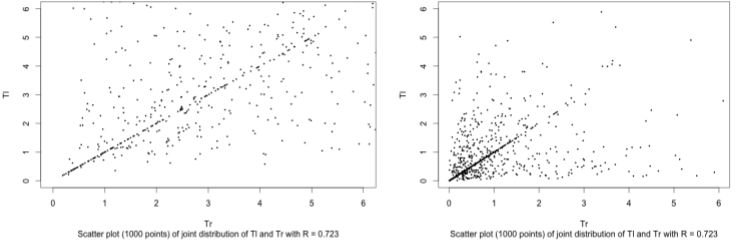
\includegraphics[width=1.0\textwidth]{Dst_height.png}
%\caption{Distribution of different tree heights, generated from simulated runs of the Markov model for the recombination-only and the recombination and migration model.}
%\label{Figure: n = 3 lumped recomb}
%\end{figure}

%
%\subsection{The lumped model and $n = 3$.}
%
%Partitioning a Markov chain into subsets of states, also referred to as ``lumping" a Markov chain, reduces the number of states. A continuous-time Markov chain is lumpable with respect to a partition if and only if, for any subsets $T_i$ and $T_j$ in the partition, and for any states $n$, $n'$ in subset $T_i$, where $P(i,j)$ is the transition probability from state $i$ to state $j$,
%\begin{equation}
%\sum_{m \in T_j} P(n, m) = \sum_{m \in T_j} P(n', m)
%\label{Eqn: lumpability}
%\end{equation}
%
%Similarly, the same condition holds for rates instead of probabilities when the Markov chain is continunous time.
%
%Lumpability is useful in this project to reduce the size of state-space due to the different symmetries which can be ignored: the transitions and states are respectively the same for each locus (right or left) and each population (A or B) and transitions to symmetric states are mutually exclusive.
%
%The lumped space from the \cite{SimonsenChurchill1997} model can be used to elucidate the state space of $n=3$, without population structure. State-space represented in its ``lumped" space can be deconstructed into the unlumped space. 
%
%It may be possible to ``un-lump" the $n=3$ model to include topology, which could be interesting for combining with the \cite{SlatkinPollack2008}

%% Lumping -- easier to add migration, add add topology for n =3
%% n = 3 (lumpy space)

% Hudson, R. R. 1983. Properties of a neutral allele model with intragenic recombination, Theoretical Population Biology 23, 183-201.

% Hudson, R. R. 1990. Gene genealogies and the coalescent process, Oxford Suverys in Evolutionary Biology 7, 1-44.

% Dutheil, Julien Y., et al. Ancestral Population Genomics: The Coalescent Hidden Markov Model Approach. Genetics 183 (2009): 259-74. 

% Griffiths, R. C. 1981. Neutral two-locus multiple allele models with recombination, Theoretical Population Biology 19, 169-186.

%\begin{figure}[ht]
%\centering
%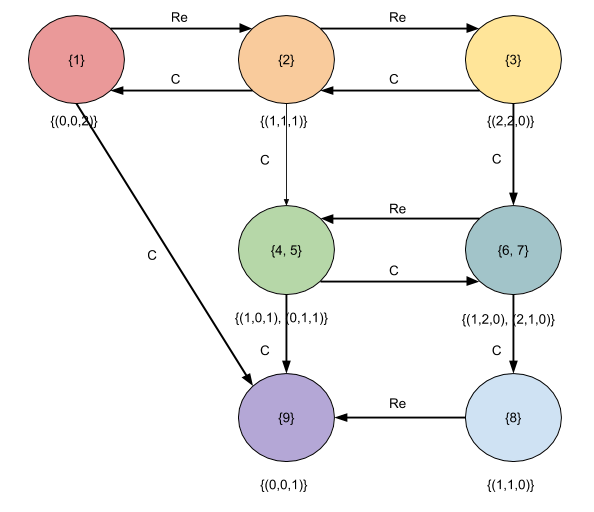
\includegraphics[width=0.5\textwidth]{Lumped_recomb.png}
%\caption{Lumped Markov chain in model with recombination, no substructure.}
%\label{Figure: lumped recomb}
%\end{figure}
%
%\begin{figure}[ht]
%\centering
%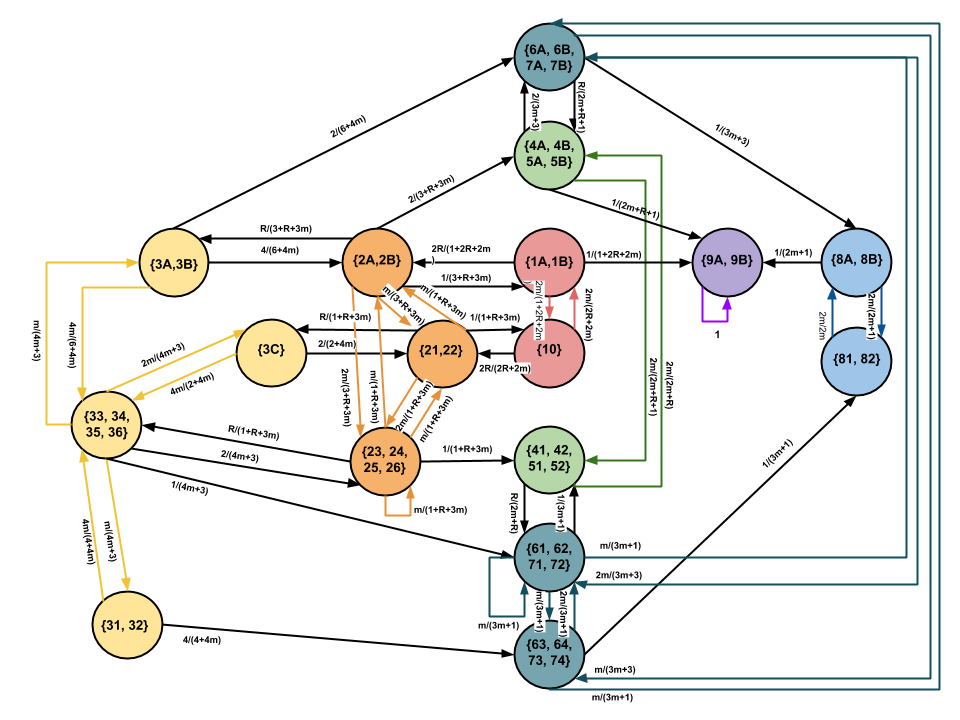
\includegraphics[width=1.00\textwidth]{Lumped_RecombMig.png}
%\caption{Lumped Markov chain in model with recombination and substructure.}
%\label{Figure: lumped recomb mig}
%\end{figure}
%
%\begin{figure}[ht]
%\centering
%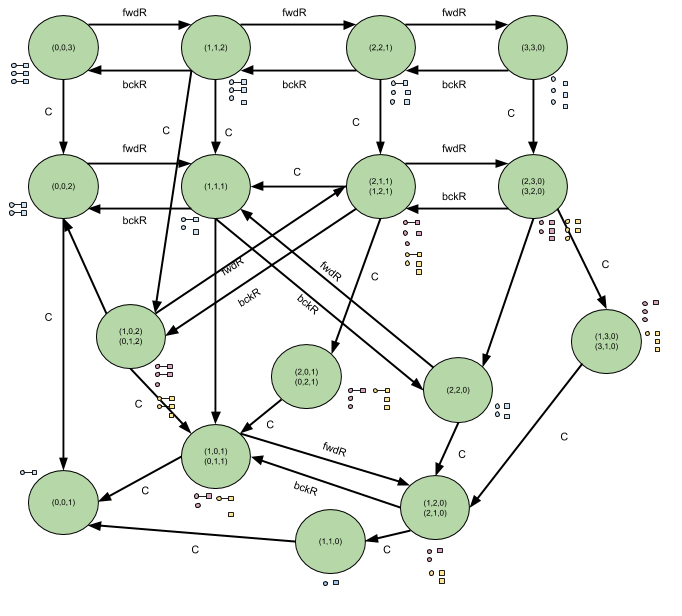
\includegraphics[width=1.0\textwidth]{n3_notopology_lumped_recomb.png}
%\caption{Lumped state space for $n = 3$ with recombination, no substructure.}
%\label{Figure: n = 3 lumped recomb}
%\end{figure}

\clearpage

\vskip .4cm
\begin{small}
\bibliographystyle{chicago}
\bibliography{Markov_ReMig.bib}
%\bibliographystyle{plainnat}
%\bibliography{Intro}
\end{small}

%% FIgure 1
\begin{figure}[ht]
\centering
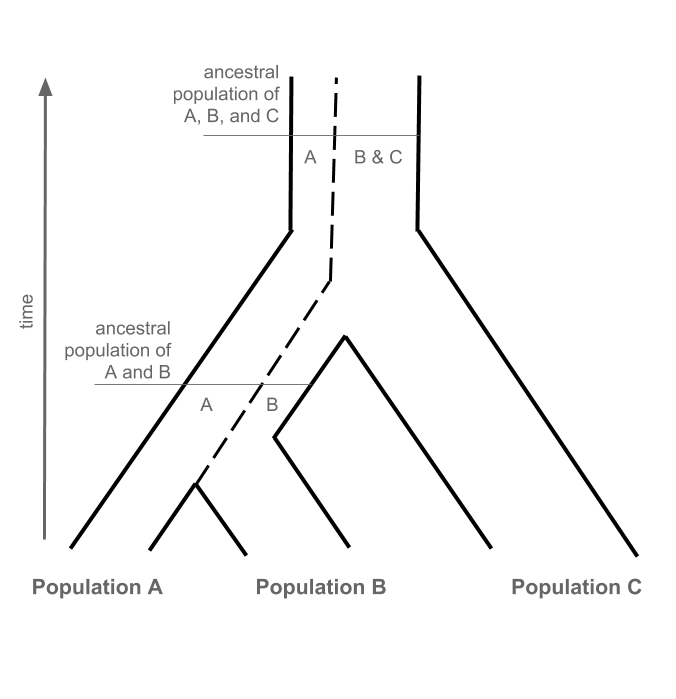
\includegraphics[width=0.75\textwidth]{SlatkinPollack2008.png}
\caption{A simple demographic history between three populations in which population substructure leads to an increase in the probability of gene-species tree discordance compared to a model without substructure \citep{SlatkinPollack2008}.}
\label{Figure: Slatkin and Pollack 2008}
\end{figure}

%% Figure 2
\begin{figure}[ht]
\centering
\captionsetup[subfigure]{justification=centering}
    \begin{subfigure}{.45\textwidth}
        \centering
        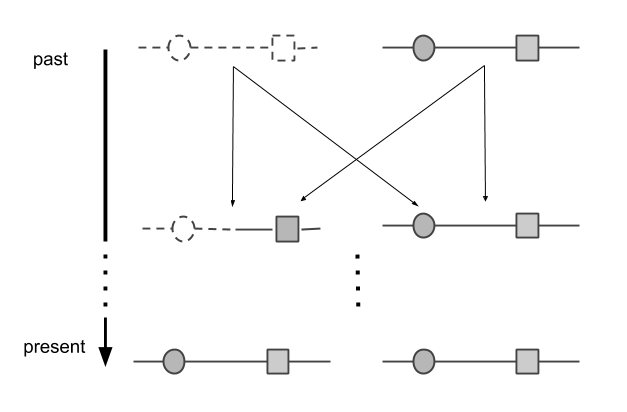
\includegraphics[width=\linewidth]{coalescence.png} 
        \caption{Coalescence} 
    \end{subfigure} %
    \begin{subfigure}{.45\textwidth}
        \centering
        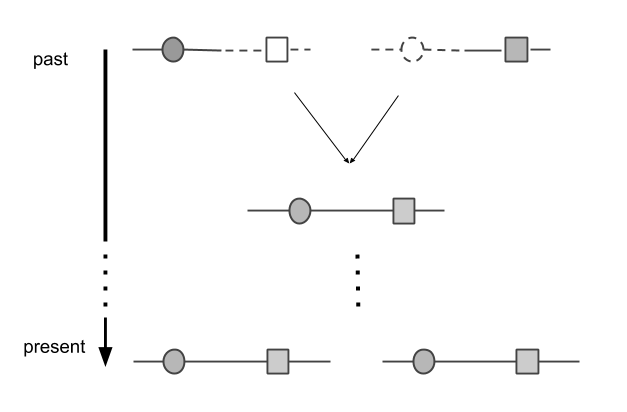
\includegraphics[width=\linewidth]{recombination.png}
        \caption{Recombination}
    \end{subfigure} 
\caption{Coalescence and recombination for pairs of loci. Consider the light gray shapes as the loci that are ancestral to the present-day sample, and consider empty shapes as loci that are not ancestral. The circle and square represent two loci of interest. In a model with recombination, looking backwards in time, the loci that are ancestral to the present-day sample can coalesce onto the same haplotype or can recombine away from each other. (A) An individual can produce offspring who inherit both loci or only one locus of interest. (B) Lineages ancestral to the present-day sample at different loci can recombine onto the same haplotype.} 
\label{Figure: coalescence and recombination}
\end{figure}

%% Figure 3
\begin{figure}[ht]
\centering
\captionsetup[subfigure]{justification=centering}
    \begin{subfigure}{.3\textwidth}
        \centering
        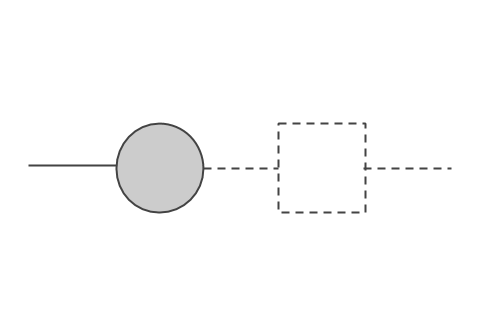
\includegraphics[width=\linewidth]{Left_type.png} 
        \caption{Left type} 
    \end{subfigure} %
    \begin{subfigure}{.3\textwidth}
        \centering
        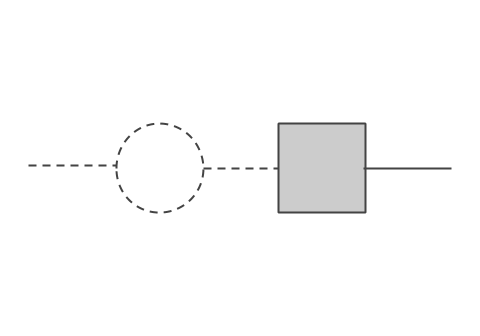
\includegraphics[width=\linewidth]{Right_type.png}
        \caption{Right type}
    \end{subfigure} 
    \begin{subfigure}{.3\textwidth}
        \centering
        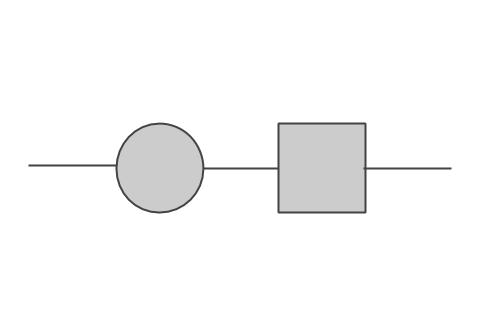
\includegraphics[width=\linewidth]{Double_type.png}
        \caption{Double type}
    \end{subfigure} 
\caption{Ancestral loci in a two locus model. The states of the Markov chain are determined by the unique tuple denoting the number of ``right type", ``left type", and ``double type" locus pairs. For an individual, the gray shapes represent loci ancestral to the present-day sample.} 
\label{Figure: terminology}
\end{figure}

% Figure 4
\begin{figure}[ht]
\centering
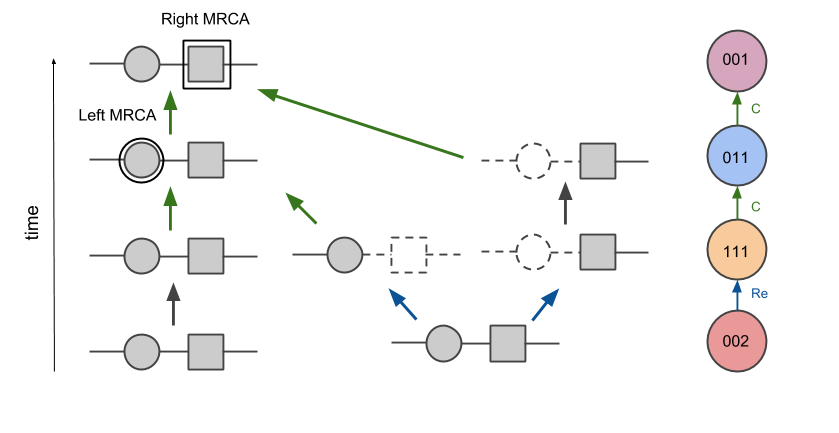
\includegraphics[width=1.00\textwidth]{Recombination_diagram.png}
\caption{An illustrative example of a process that traces the lineages of two loci for two individuals. Recombination and coalescence can change the number of lineages of each type in each population. In this case, the tree associated with left loci is shorter than the tree associated with the right loci.}
\label{Figure: recombination diagram}
\end{figure}

% Figure 5
\begin{figure}[ht]
\centering
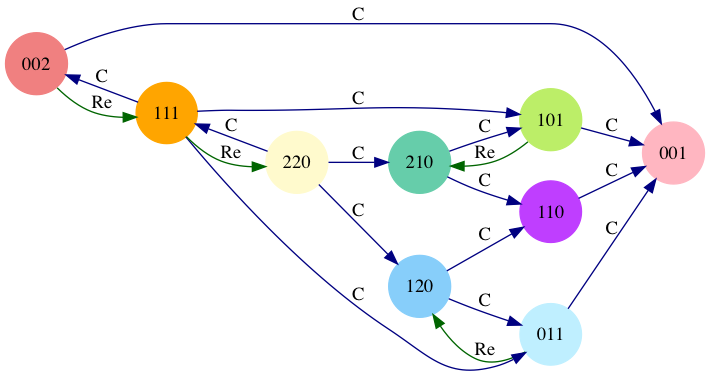
\includegraphics[width=0.75\textwidth]{n2_recomb_color.png}
\caption{State space with transitions for $n = 2$ with recombination but no population substructure (recreation of Figure 3 from \cite{SimonsenChurchill1997}) Each triplet $ijk$ gives the number of left, right, and double lineages in a state respectively. C indicates a coalescent event to transition between states and Re represents a recombination event to transition between states. The process begins in state 002 and proceeds to coalescence in state 001}
\label{Figure: n = 2 recomb}
\end{figure}

% Figure 6
\begin{figure}[ht]
\centering
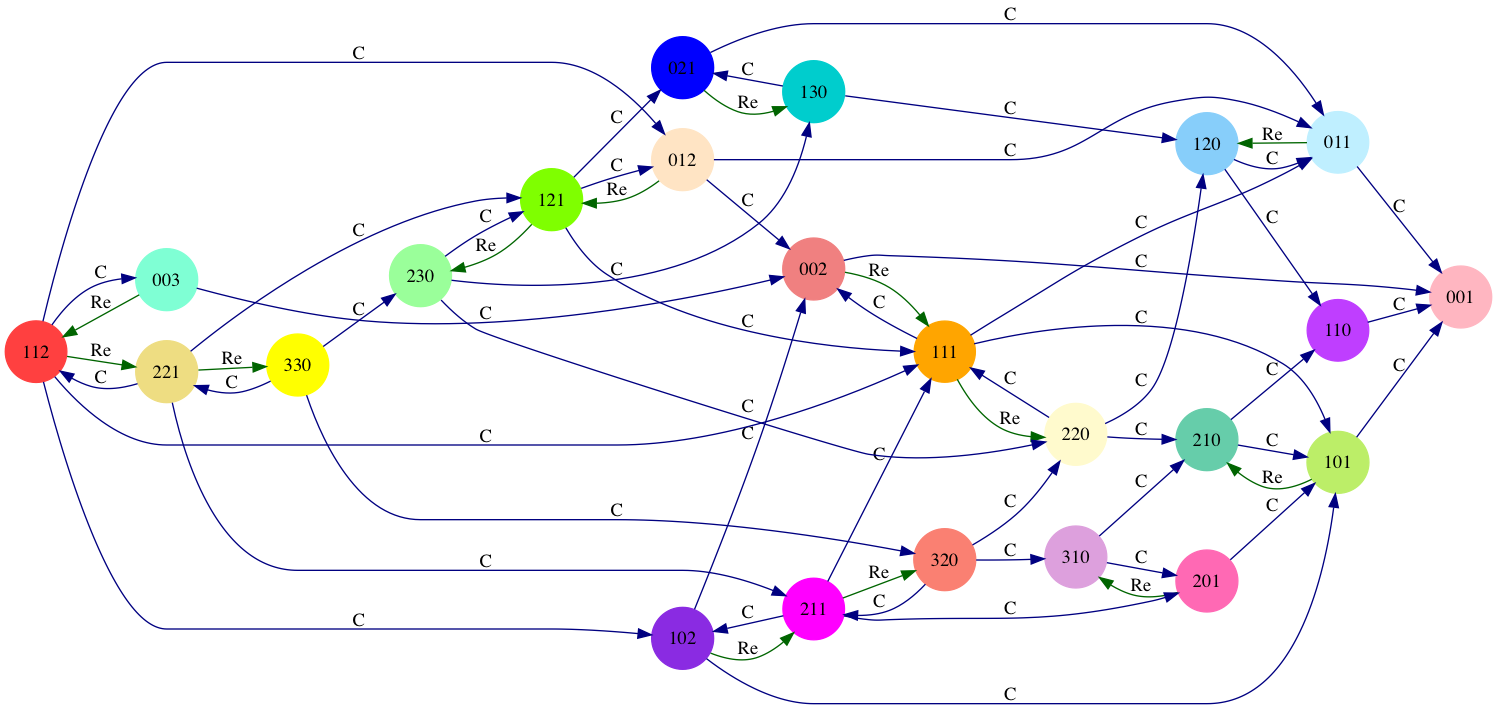
\includegraphics[width=1.00\textwidth]{n3_recomb_color.png}
\caption{The model of \cite{SimonsenChurchill1997} with $n = 3$. The model has recombination but no population substructure. The 9 states of the $n = 2$ case also appear in the model with $n = 3$. The colors of the states are consistent between this figure and Figure \ref{Figure: n = 2 recomb}, to illustrate how the $n = 2$ chain is embedded in the state space of $n = 3$.}
\label{Figure: n = 3 recomb}
\end{figure}

% Figure 7
\begin{figure}[ht]
\centering
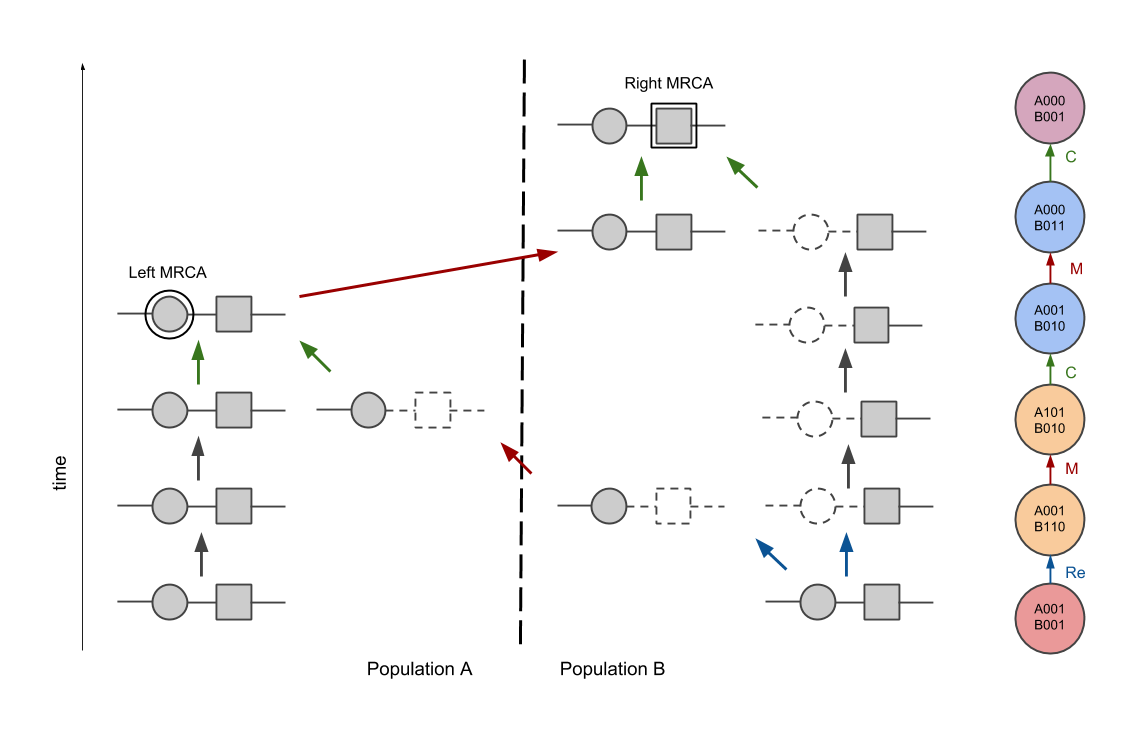
\includegraphics[width=1.00\textwidth]{Migration_diagram.png}
\caption{An illustrative example of a process that traces the lineages of two loci for two individuals in two populations. Recombination, migration, and coalescence can change the number of each lineage type in each population. In this case, the tree associated with left locus is shorter than the tree associated with the right locus.}
\label{Figure: migration diagram}
\end{figure}

% Figure 8
\begin{figure}[ht]
\centering
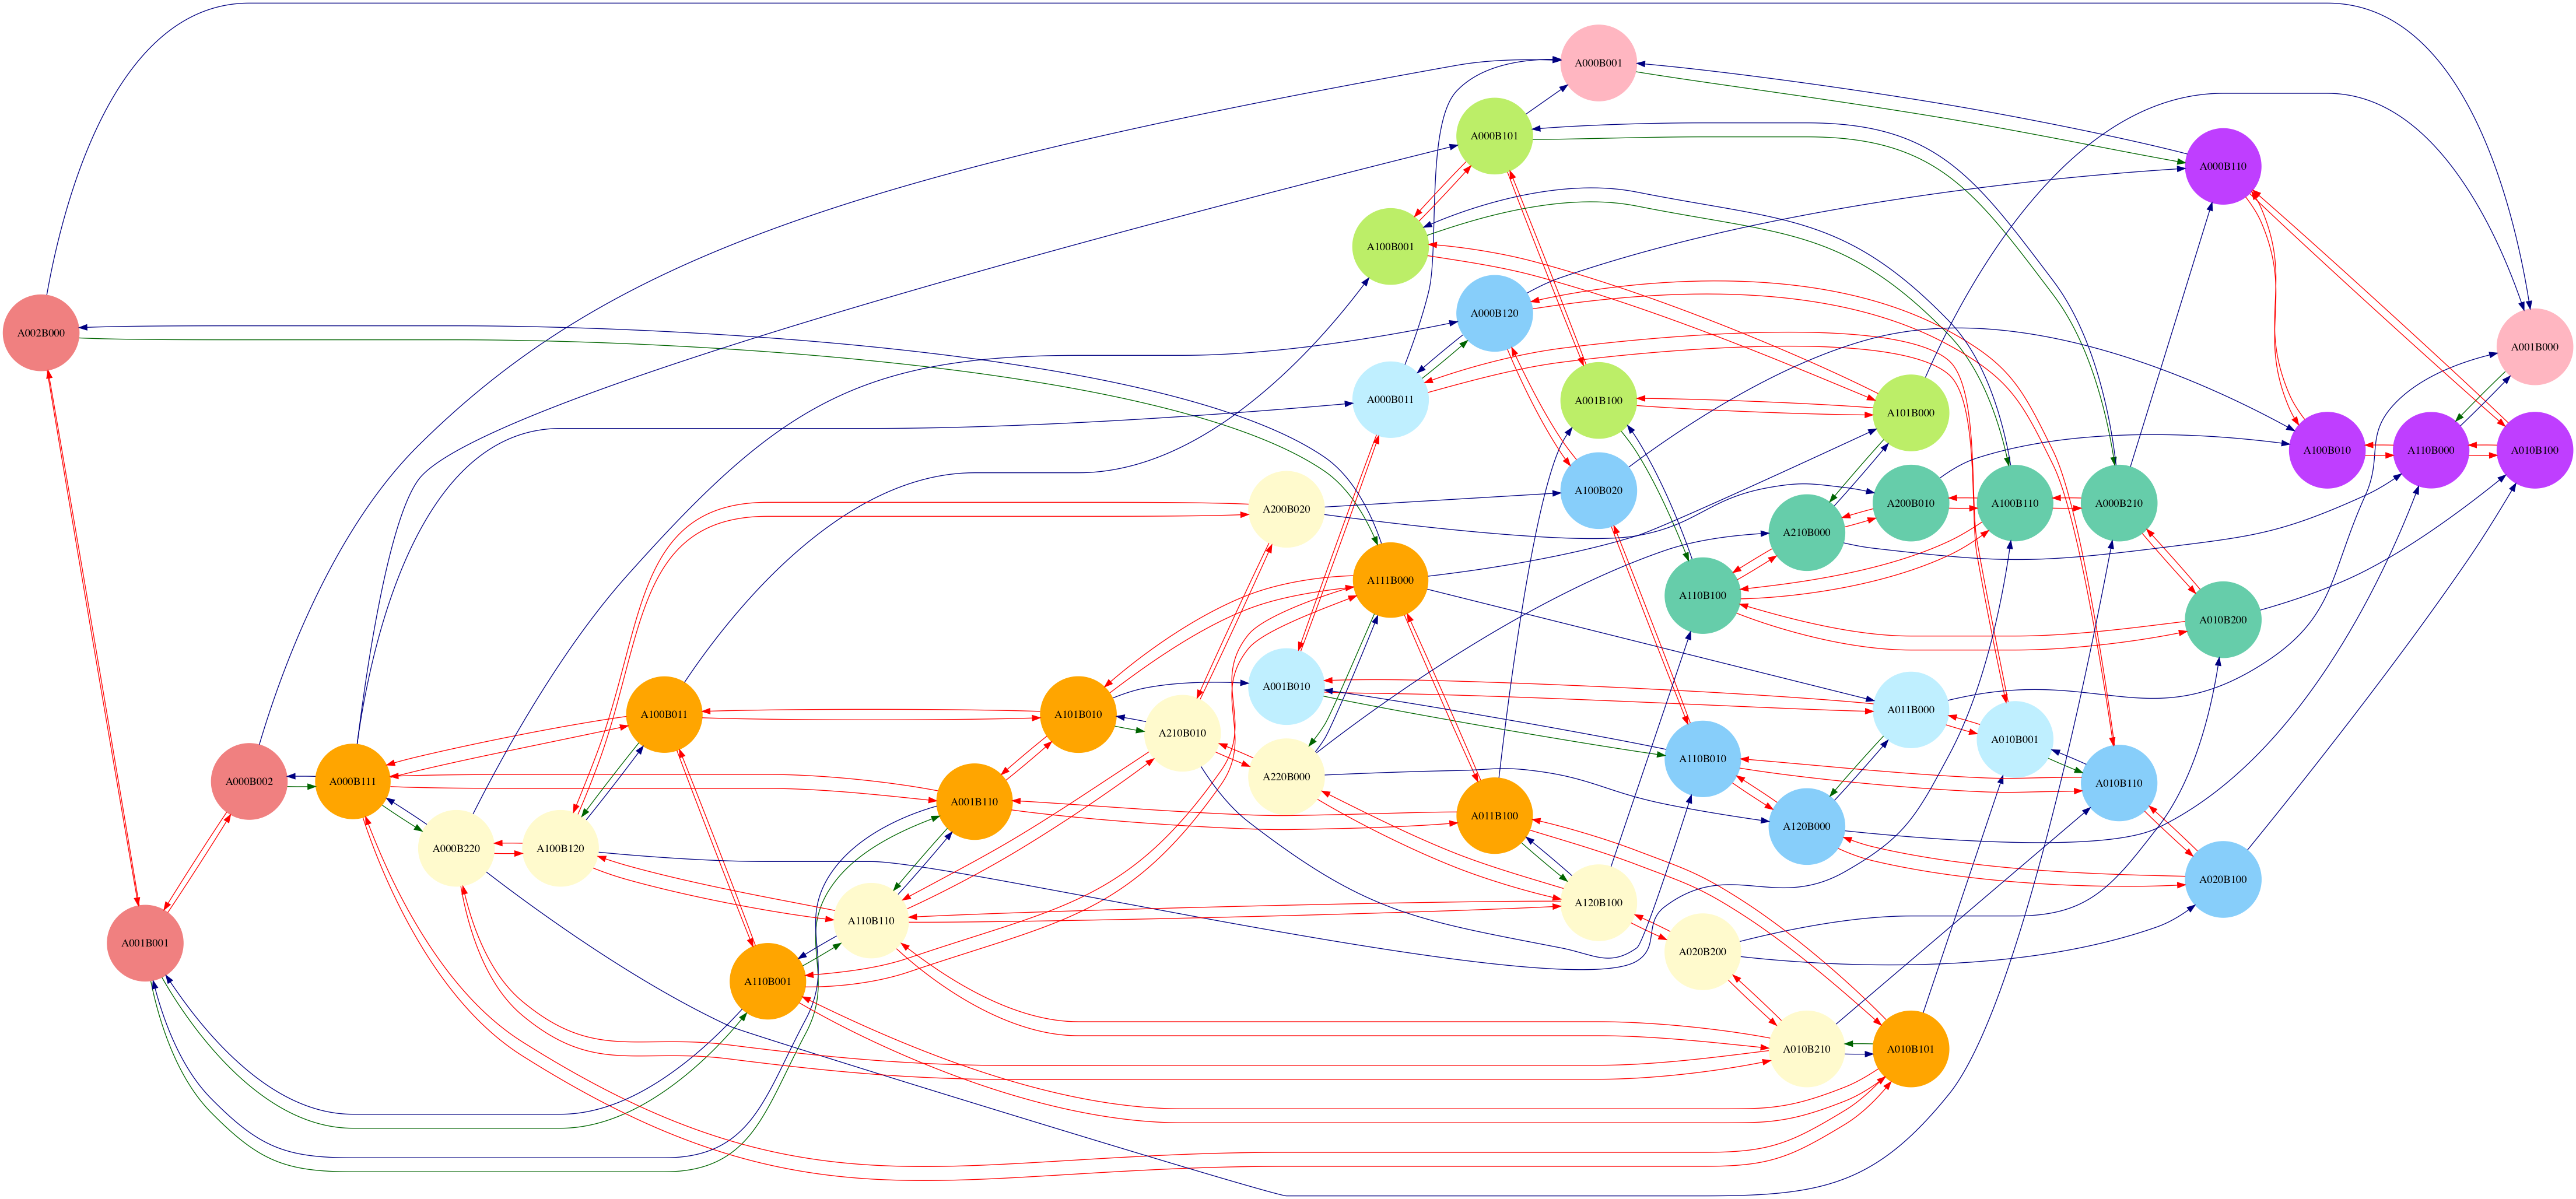
\includegraphics[width=\hsize]{n2_mig_color.png}
\caption{Full state space and transitions for $n = 2$, model with recombination and migration. The number of states is 46. Coalescence events are represented by blue lines. Recombination events are represented by green lines. Migration events are represents by red lines. The colors of states corresponds to the states in the recombination only model if the population labels are removed.}
\label{Figure: n = 2 recomb mig}
\end{figure}

% Figure 9
%\begin{figure}[ht]
%\raggedleft
%\includegraphics[width=1.0\textwidth]{n3_mig_color.png}
%\caption{Full state space and transitions for $n = 3$, model with recombination and migration. The number of states is 184. Coalescence events are represented by blue lines. Recombination events are represented by green lines. Migration events are represents by red lines. The colors of states corresponds to the states in the recombination only model with only recombination and no population substructure.}
%\label{Figure: n = 3 recomb mig}
%\end{figure}

% Figure 10
\begin{figure}[ht]
\centering
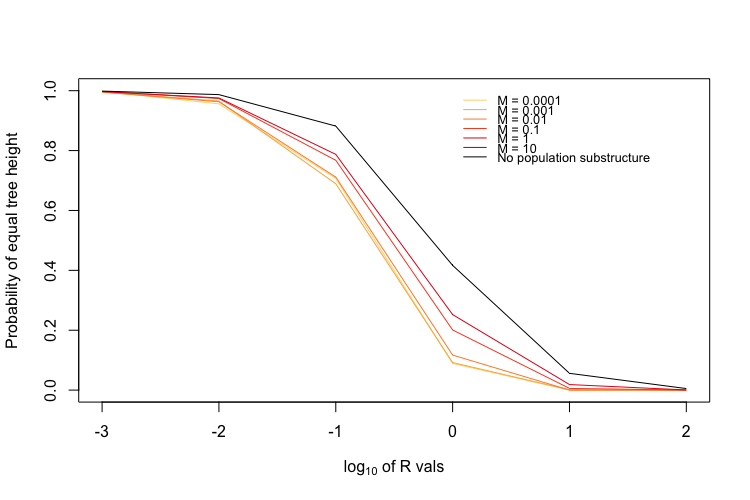
\includegraphics[width=0.75\textwidth]{pequalht.png}
\caption{Probability of equal tree heights for different migration rates, $2Nm = M$ and recombination rates, $2Nr = R$.  estimated from $10^4$ simulations of the Markov process}
\label{Figure: pequal height}
\end{figure}


\end{document}